\documentclass[11pt, oneside]{article}   	% use "amsart" instead of "article" for AMSLaTeX format
\usepackage{geometry}                		% See geometry.pdf to learn the layout options. There are lots.
\usepackage{textcomp}
\usepackage[colorlinks=true,urlcolor=blue]{hyperref} 
\geometry{letterpaper}                   		% ... or a4paper or a5paper or ... 
\usepackage[parfill]{parskip}    		% Activate to begin paragraphs with an empty line rather than an indent
\usepackage{graphicx}				% Use pdf, png, jpg, or eps§ with pdflatex; use eps in DVI mode
								% TeX will automatically convert eps --> pdf in pdflatex		
\usepackage{amssymb}
\usepackage{amsmath}
\usepackage{relsize}

\usepackage{tikz}
\usetikzlibrary{arrows,automata}
\usetikzlibrary{positioning}


\tikzset{
    state/.style={
           rectangle,
           rounded corners,
           draw=black, very thick,
           minimum height=2em,
           text centered,
           },
}

\title{CS181 / CSCI E-181 Spring 2014 Final Project}
\author{
  David Wihl\\
  \texttt{davidwihl@gmail.com}
  \and
  Zachary Hendlin\\
  \texttt{zgh@mit.edu} 
}
%\date{}							% Activate to display a given date or no date


\begin{document}
\maketitle

\begingroup
\hypersetup{linkcolor=blue}
\tableofcontents
\endgroup

\section{Introduction}
Creating an agent to play Pacman required us considering a number of steps:
(1) Determining the latent class that each ghost belongs to based on its features (classification)
(2) Analyzing / visualizing the juciness of ghost by class (simple data analysis)
(3) Classification of capsule class (e.g. placebo or immunity to eating bad ghosts)
(4) A decision rule for the Pacman, either 'harded coded' or 'learned' (e.g. q-learning, policy interation, hidden markov models)

\section{Classification of Ghosts}
To gather sufficient data, we allowed the SampleAgent (provided intially in the code) to play until ~30 megabytes of ghost training data was captured on, to get data on feature vectors and associated 'juciness' point values of each.

We sought to classify ghosts as \{0, 1, 2, 3, 5\}, where all ghosts in category 5 are dangerous (e.g. induce a reward of -1000 points unless a helpful capsule is consumed first). Because of the huge payoff in eating a helpful capsule and then eating a 'bad' ghost, this is extremeley important.

We explored two methods for classifying the ghosts on the basis of their features.

First, we explored linear support vector machines (SVMs) using SK-Learn's Stochastic Gradient Descent classifier.

For classifying the category 5 ghosts, this approach was accurate 90.62 percent of the time. Our analysis found that while differences in the rewards associated with eating ghosts not from class 5 did differ by class, the most important thing for us to measure our performance on is the correct classification of dangerous (class 5 ghosts).

<graph here>

We also used logistic regression classification, and achieved somewhat better results, with correct classification of class 5 ghosts 93.25 percent of the time.

We elected to use the logistic regression classification results to predict which class each ghost is in during runtime.

One additional way to tell if a ghost is category 5 (and hence dangerous) is it's change in distances from the Pacman. 'Bad ghosts' generally move closer and closer to the Pacman, whereas good ghosts do not demonstrate this behavior.

\section{Estimating the Juciness of Ghosts}

We had first thought about trying to pursue the highest point value ghosts and then follow them. But it turned out that the behavior of the aggressive 'bad ghost' dominated trying to eat regular ghosts.

As such, the data bore out that eating protective capsules and then pursuing the bad ghost was the most important thing for our Pacman to go pursue.

\section{Classification of Capsules and Placebos}
We wanted to determine which of the pills are helpful capsules and which are placebos. To do this, we first plotted the helpful capsules which we collected using the '-d' data collection function.

Here we determined that capsule feature values were very much clustered into three distinct clusters as shown below.
<show graph>

This suggested that we could either fit Gaussians to these points as part of a generative approach, or apply something like K-means to find the clusters. Because the data were in three dimensions, we opted to use k-means for clustering, and initiated the model with kmeans++.

Because the three clusters were all positively identified, simply assigning a new value at run-time (for a capsule which may be a `good' or `placebo'), we instead used the `score' attribute to evaluate the distance from the centroid the data point would have been assigned to. We are agnostic to which centroid the capsule would be assigned to but we are very sensitive to the score assigned (e.g. the distance from the centroid assignment), with larger distances being worse.

From our positive training data, we found values of $0$ to $-118$ as the `good' range of objective function values. Any value $<-118$ would likely be a placebo capsule.

So at runtime we score each capsule based on its $3\times1$ feature vector and we consider the `best' capsule the one with the maximum objective function value when scored.

\section{Decision Rules}

\subsection{Reinforcement Learning}
We first attempted to implement a Q-learning based approach, but very quickly found this to be infeasible due to the extremely large state space.

For a 20x20 matrix five ghosts (each with a class of 1 to 5), five capsules (each with a 1/0 classification), and our Pacman's ability to make four moves, our (state, action) space is (20^2)^5 ^5 * (20^2)^5 ^2 * (20^2) *4.

It is clear that we get to such a large state space that we can't reasonably visit every single state. We tried to reduce the state space by only keeping track of the 'good' capsules and the 'bad' ghosts but we still found this state space to be too large to fit. 

Although we coded up Q-learning, ran it for a while, and tried to reduce the dimensionality of the state space, we still found this state space to be too large.

\subsection{Rules Engine}
Our next approach was to build a procedural rules engine inspired by a Markov process. In other words, the rules engine did not require any historical data and would simply decide the next action based on the current state of the game.

The other reason for building a rules engine was to better grapple with the game dynamics to see if the model could be significantly simplified. We believe we were successful as the game came down to a straightforward finite state machine. 

We iterated through more than 10 different heuristics. Our average score over 50 games went from a dismal $-7390$ to a reasonable $933$.


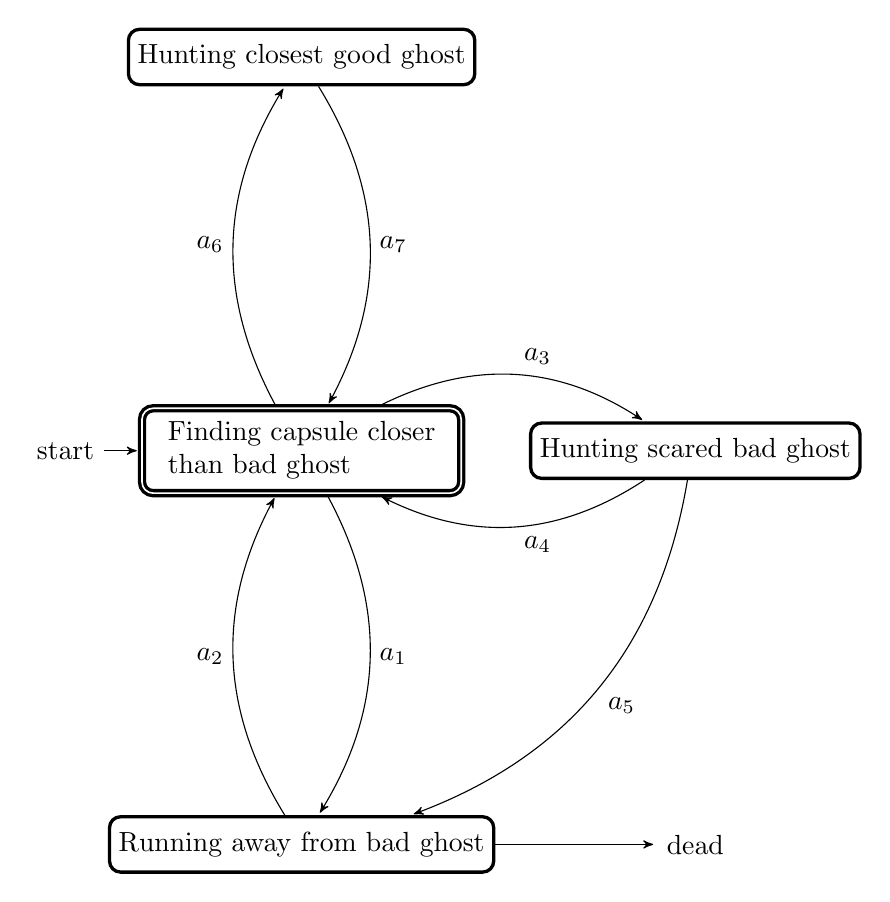
\begin{tikzpicture}[>=stealth',shorten >=1pt,auto,node distance=5cm]
 	\tikzstyle{every state}=[align=center]

	\node[initial,state,accepting] (S1)      
			{
				\begin{tabular}{l}
				Finding capsule closer\\
				than bad ghost
				\end{tabular}
			};
	\node[state]         (S2) [below of=S1]  {Running away from bad ghost};
	\node[state]         (S3) [right of=S1] {Hunting scared bad ghost};
	\node[state]	   (S4) [above of=S1] {Hunting closest good ghost};
	\node[state,draw=none,fill=none]	   (die) [right of=S2] {dead};
	
	\path[->] (S1) edge  [bend left]           node  {$a_3$} (S3);
	\path[->] (S3) edge  [bend left]           node {$a_4$} (S1);
	
	\path[->] (S1) edge  [bend left]           node [align=right] {$a_1$} (S2);
	\path[->] (S2) edge  [bend left]           node {$a_2$} (S1);
	
	\path[->] (S3) edge [bend left]          node {$a_5$} (S2);
	
	\path[->] (S1) edge  [bend left]           node {$a_6$} (S4);
	\path[->] (S4) edge  [bend left]           node {$a_7$} (S1);

	\path[->] (S2) edge node {} (die);
	
\end{tikzpicture}

where:
\begin{description}
	\item[$a_1$] bad ghost closer than good capsule
	\item[$a_2$] good capsule closer than bad ghost
	\item[$a_3$] bad ghost is scared and within range
	\item[$a_4$]bad ghost is out of range
	\item[$a_5$]bad ghost will no longer be scared soon
	\item[$a_6$]no good capsule in range
	\item[$a_7$]good capsule now in range
\end{description}


The Rules engine provided the following advantages:
\begin{description}
	\item[Key Factors]We could distill key factors that would be difficult if not impossible to discover by exploration.
	\item[Latent Factors]One of the key pieces of information was the time remaining before scared bad ghost reverted to normal. We found this by careful examination of the game code. It would have been difficult if not impossible to discover this feature by exploration.
	\item[No history]Since the game changes significantly from one time click to another, a probabilistic model may take time to re-learn the new board. With our ghost and capsule classifiers, we could immediately evaluate the best option from the current board.
	\item[Flexibility]Since only the current state is necessary our rules engine would be flexible enough to handle more dynamics than in the current game. The entire board could resize,  walls could move, capsules could be in motion and the bad ghost could change between time clicks and the rules engine would still find the best course of action.
\end{description}

\section{Parameter Tuning}

\section{Other Methods}
\subsection{Expectimax}
tree would not be deep to merit this. 

\subsection{Alpha-Beta Search}
Russell \& Norvig, pg 166

\subsection{Hidden Markov Model}
 Roland Memisevic
 http://www.iro.umontreal.ca/~memisevr/code/hmm.py

Needed to find a HMM implementation that respected the dependencies of the game cluster. (For example could not use GHMM www.ghmm.org due to a C library dependency)

\section{Conclusion}
A combination of ML and traditional techniques is more powerful than using one set of techniques alone.

\begin{thebibliography}{1}

 \bibitem{item1}\emph{Reinforcement Learning}, Sutton \& Barto, 1998, ISBN-10: 0-262-19398-1
 
  \end{thebibliography}

\end{document}  
